\documentclass[spanish]{article}
\usepackage[T1]{fontenc}
\usepackage[utf8]{inputenc}

\normalsize

\parindent = 0mm 

\usepackage{lmodern}
\usepackage[a4paper]{geometry}
\usepackage[spanish]{babel}
\usepackage{graphicx}
\usepackage{url}
\usepackage{booktabs}
\usepackage{multicol}
\usepackage{multirow}
\usepackage[x11names,table]{xcolor}
\usepackage{amsmath, latexsym, amsfonts, amssymb} 
\usepackage{multicol}
\usepackage[shortlabels]{enumitem}
\usepackage{tikz}
\usepackage{floatrow}
\usepackage[small,bf,labelsep=period]{caption}
\usepackage[backend=biber]{biblatex}

\usepackage{bera}
\usepackage{listings}
\usepackage{xcolor}

\colorlet{punct}{red!60!black}
\definecolor{background}{HTML}{EEEEEE}
\definecolor{delim}{RGB}{20,105,176}
\colorlet{numb}{magenta!60!black}

\lstdefinelanguage{json}{
    basicstyle=\normalfont\ttfamily,
    numbers=left,
    numberstyle=\scriptsize,
    stepnumber=1,
    numbersep=8pt,
    showstringspaces=false,
    breaklines=true,
    frame=lines,
    backgroundcolor=\color{background},
    literate=
     *{0}{{{\color{numb}0}}}{1}
      {1}{{{\color{numb}1}}}{1}
      {2}{{{\color{numb}2}}}{1}
      {3}{{{\color{numb}3}}}{1}
      {4}{{{\color{numb}4}}}{1}
      {5}{{{\color{numb}5}}}{1}
      {6}{{{\color{numb}6}}}{1}
      {7}{{{\color{numb}7}}}{1}
      {8}{{{\color{numb}8}}}{1}
      {9}{{{\color{numb}9}}}{1}
      {:}{{{\color{punct}{:}}}}{1}
      {,}{{{\color{punct}{,}}}}{1}
      {\{}{{{\color{delim}{\{}}}}{1}
      {\}}{{{\color{delim}{\}}}}}{1}
      {[}{{{\color{delim}{[}}}}{1}
      {]}{{{\color{delim}{]}}}}{1},
}


\bibliography{referencias}

\title{Manual de Usuario\\
    \large Construcción y graficación de grafos causales}

\author{ Dennis Fiallo Muñoz \\ Lauren Guerra Hernández}
\date{}

\begin{document}
\maketitle

\section*{Presentación de Interfaz Visual}

La interfaz visual se va a dividir en dos partes principales:
\begin{itemize}
    \item \textbf{La Barra de Opciones:} Se encuentra a la izquierda. Esta contiene un conjunto de opciones que se le dan al usuario de las que se van a estar ablando más adelante.
    \item \textbf{La Ventana de Construcción:} Es el lugar donde se van a mostrar los grafos causales generados según la información dada.
\end{itemize}

\begin{figure}[H]
    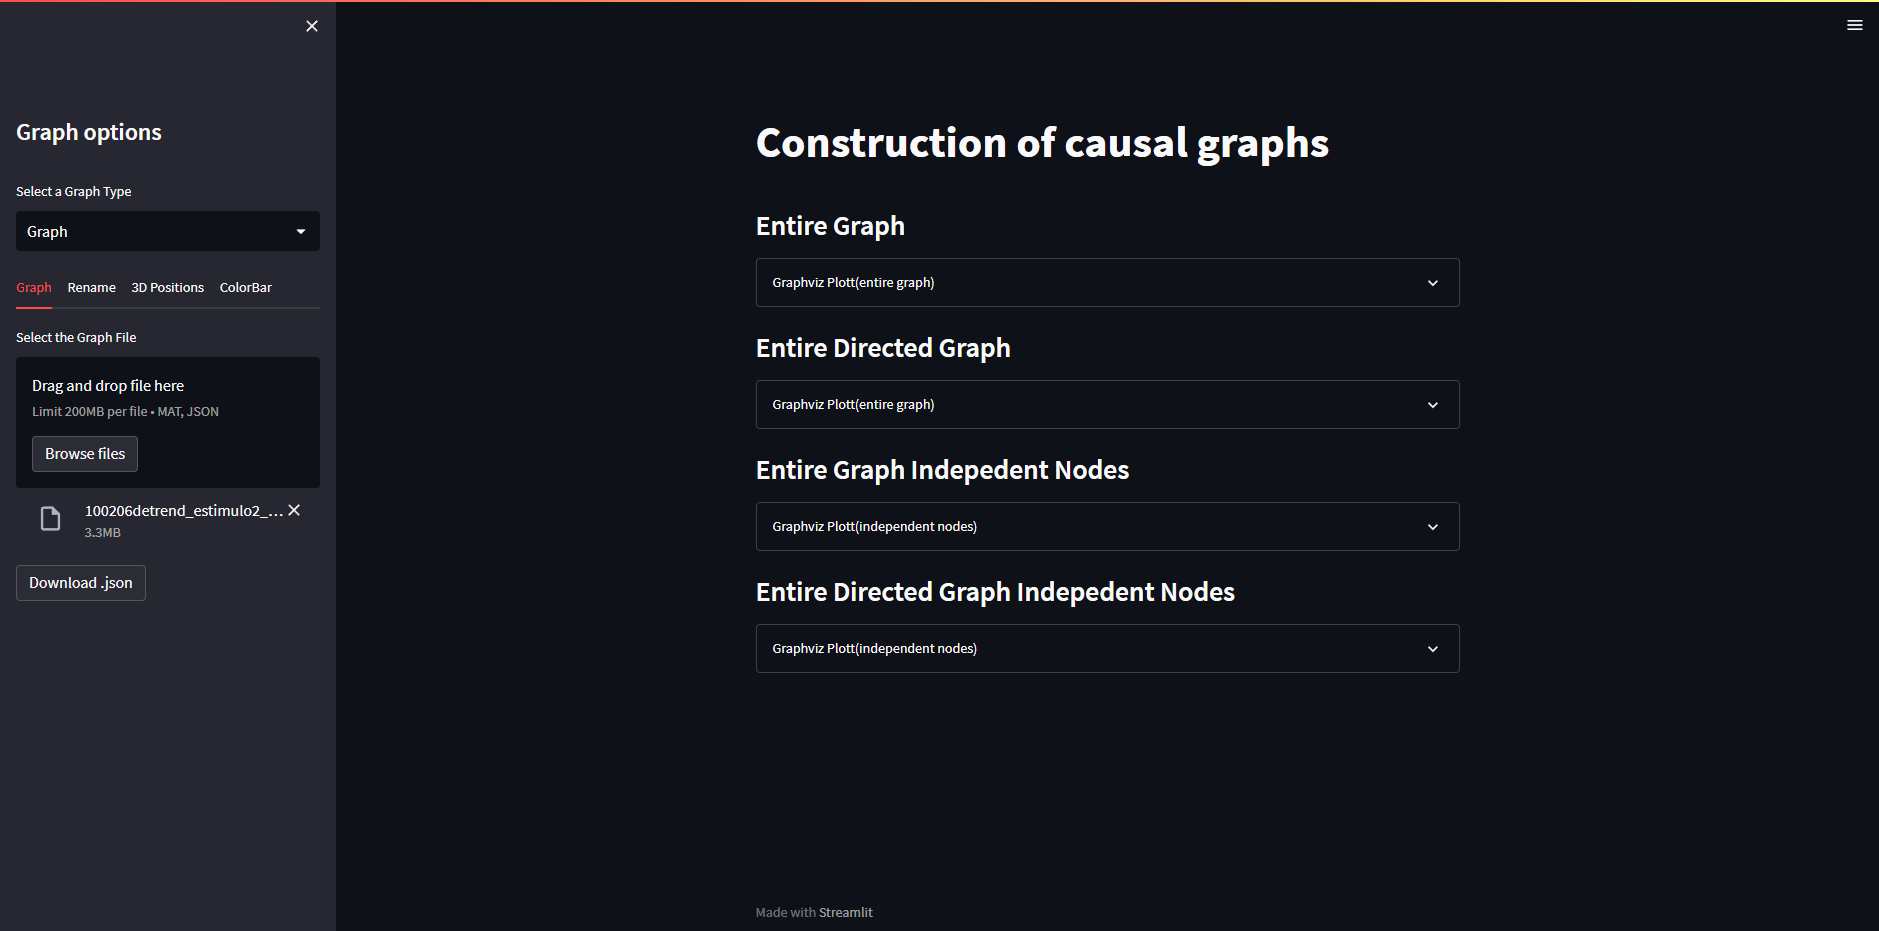
\includegraphics[scale=0.20]{visual.png}
\end{figure}	


\section*{Barra de Opciones}

\subsection*{Tipos de Grafos}
En esta aparece primeramente un SelectBox con 3 distintas opciones de modelo de graficado:

\begin{itemize}
    \item \textbf{Graph:} Presenta el modelo más simple de visualización pero más estable y capaz de guardar imágenes de los grfos con mayor calidad. En este se presenta el grafo no dirigido(lag 0), el grafo dirigido(resto de lags), además de la opción de seleccionar nodos independientes de cada grafo y mostrarlos.
    \item \textbf{Complex Graph:} Un modelo con métodos de graficado más complejos, permitiendo alternar entre algoritmo como Atlas 2 o Hierarchical Repulsion. Sin embargo las images que guarda son de menor calidad. Posee las mismas opciones de visualización que el caso anterior.
    \item \textbf{3D Graph:} En este se muestran los grafos en un espacio tridimensional, usando las ubicaciones a escala de los nodos que se representan.
\end{itemize}

\subsection*{Entrada de Datos}

\subsubsection*{Graph}

Se admite como entrada archivos .mat que contengan un diccionario, teniendo como llaves linkLag y vallag enumerados desde 0 hasta n(Ejemplo: linkval0, linkval1, linval2, ….) y teniendo como contenido la matriz correspondiente a este. También se admiten .json con el siguiente formato:


\begin{lstlisting}[language=json,firstnumber=1]
    {
        "graph": {
            "graph":{
                "metadata": {},
                "directed": False,
                "nodes": {},
                "edges": []
            }
        },
        "digraph": {
            "graph":{
                "metadata": {},
                "directed": True,
                "nodes": {},
                "edges": []
            }
        }
            
    }
    \end{lstlisting}


\subsubsection*{Descargar .json}

Botón para descargar la información de los grafos que se usa en la aplicación en formato .json.


\subsubsection*{Rename}

Aquí se puede seleccioanr el archivo .json para cambiarle el nombre a los nodos. Estos deben tener el siguiente formato:\\

\begin{lstlisting}[language=json,firstnumber=1]
    {
        "node id": "new name",
    }
\end{lstlisting}

Se muestra un ejemplo en la carpeta data con el nombre de $rename\_nodes.json$.


\subsubsection*{3D Positions}

Se puede seleccionar un archivo .json para definir las posiciones espaciales de los nodos. Debe presentar el siguiente formato:

\begin{lstlisting}[language=json,firstnumber=1]
    {
        "node id": {
            "x": x,
            "y": y,
            "z": z,
        },
    }
\end{lstlisting}

Se muestra un ejemplo en la carpeta data con el nombre de $brain\_3d.json$.\\


\subsubsection*{Agregar Barra de Color}

Con esta opción se selecciona una de las imágenes tomadas de los grafos causales y se le agrega la barra de colores según el peso de los enlaces de los nodos. Al seleccionar la imagen aparece automáticamente una vista previa de la imagen resultante, además de un botón para descargarla.


\section*{Ventana de Construcción}

Todos los modelos traen consigo a la derecha una barra con las siguientes opciones

\begin{itemize}
    \item \textbf{General:}
    \begin{itemize}
        \item Reset: Vuelve el grafo a su estado inicial.
        \item Enter Full Screen: Mostrar en pantalla completa el grafo.
        \item Export: Descarga la imagen del tipo seleccionado.
    \end{itemize}
    \item \textbf{Data Selection:} Seleccionar, de los metadatos de cada elemento del grafo, el que se quiera mostrar en cada parte de la graficación. Viene por defecto con el nodo mostrando su id, las aristas mostrando el label(el cual contiene los lags en el caso del dirigido) y los tamaños de los nodos y aristas segun algún tipo de dato.
    \item \textbf{Nodes:} Propiedades de los nodos.
    \item \begin{itemize}
        \item Release Fixed Nodes: Opción muy útil para reordenar los nodos usando las físicas(Generalmente mejora en gran medida la representación visual).
    \end{itemize}
    \item \textbf{Node Labels:} Propiedades del texto en los nodos.
    \item \textbf{Edges:} Propiedades de las aristas
    \item \textbf{Edge Labels:} Propiedades de los textos de las aristas
    \item \textbf{Layaut Algorithm:} Permite variar los valores de las fisicas de los grafos, además de activar y desactivar tipos de fuerzas.
\end{itemize}

% \subsection*{Graph}




\end{document}